\subsubsection{Student}
The student experience from start to finish is a much more fluid process than before, take for an example a student Jack who wishes to sign up to help find himself a job for his third year compulsary industrial placement.
  \paragraph{Sign Up:}
    The first thing Jack must do is sign up to CPP 2.0, under Imperial College's organisation. He can then choose the relevant departments he is a member of (in his case only Computing), enter a valid email address, password and password confirmation.

    \begin{figure}[H]\centering
    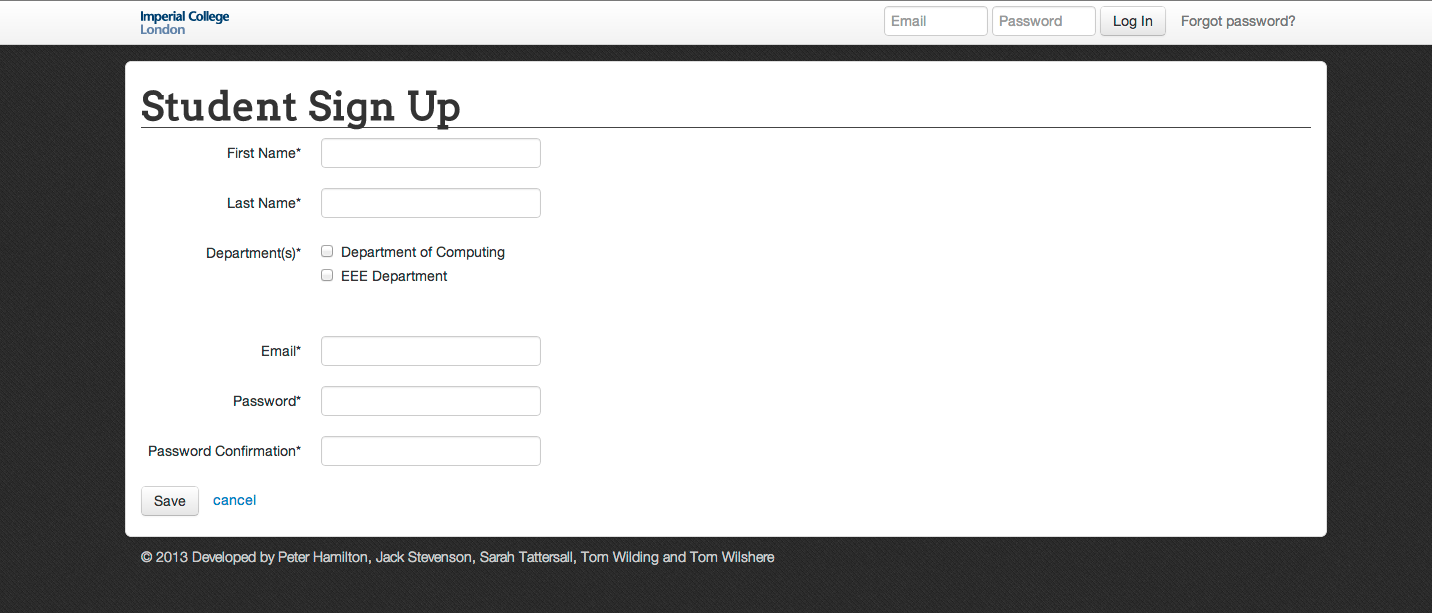
\includegraphics[scale=0.3]{images/user_experiences/student/sign_up_page}
    \caption{Student sign up view}
    \end{figure}

    In order to sign up Jack must have a valid Imperial email address which will be identified if he uses his home address. We have used this as a technique to only allow students from a particular organisation to sign up.

    \begin{figure}[H]\centering
    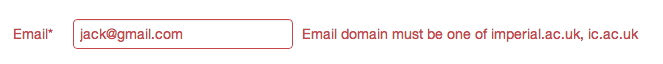
\includegraphics[scale=0.5]{images/user_experiences/student/invalid_email}
    \caption{Message displayed when student enters invalid email}
    \end{figure}

  \paragraph{Dashboard:}
    Finally when all of Jack's details are correct he procedes to his dashboard. In order to not waste companies time with students that have not filled in the minimal detail requirements we deactivate a students profile on creation. A deactivated profile will not show up in company searches and needs at minimum a year, degree, status and CV to be revealed to companies. 
    Jack is made aware of this via a drop down notifier on page load which tells him so and to make it even more obvious his student profile is greyed out with a message telling him it's deactivated.

    \begin{figure}[H]\centering
    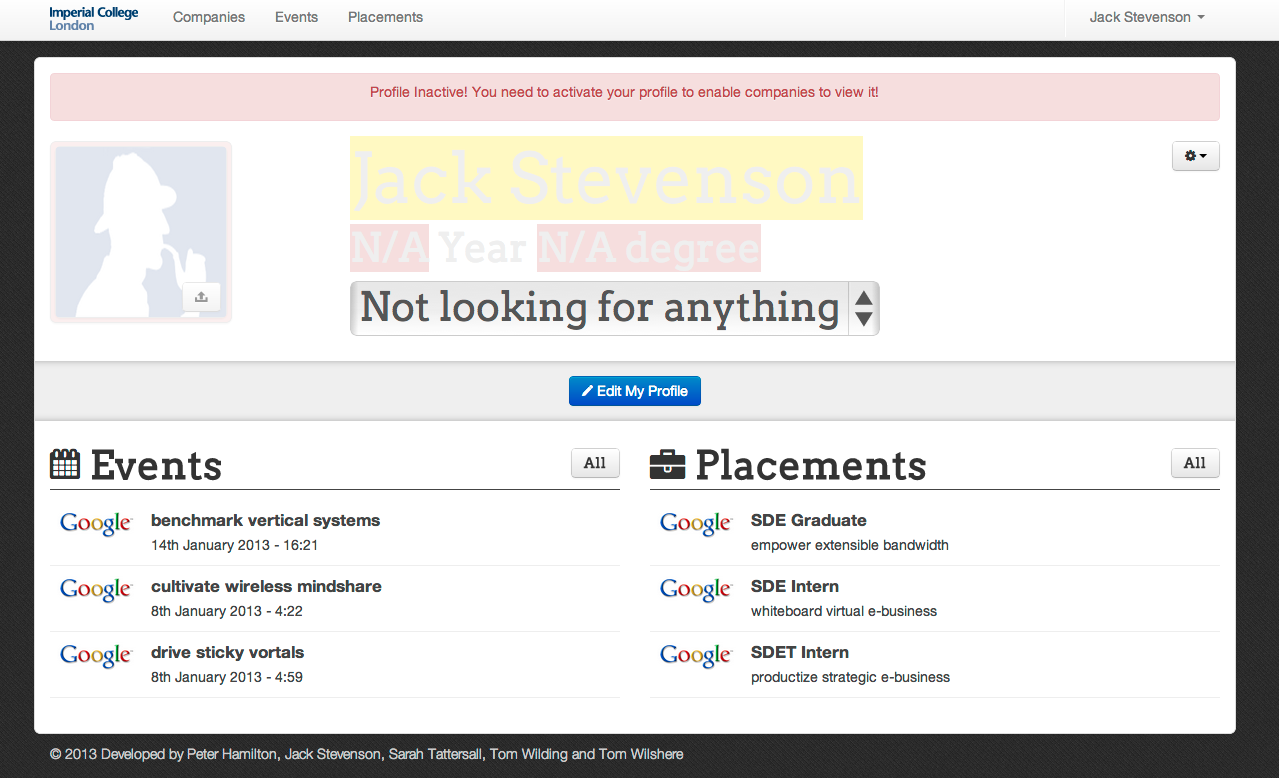
\includegraphics[scale=0.3]{images/user_experiences/student/sign_up_deactivate}
    \caption{Deactivated student profile}
    \end{figure}

    Jack can then fill in his details and activate his profile ready to be found by a company.
    A complete example of which can be seen below.
    
    \begin{figure}[H]\centering
    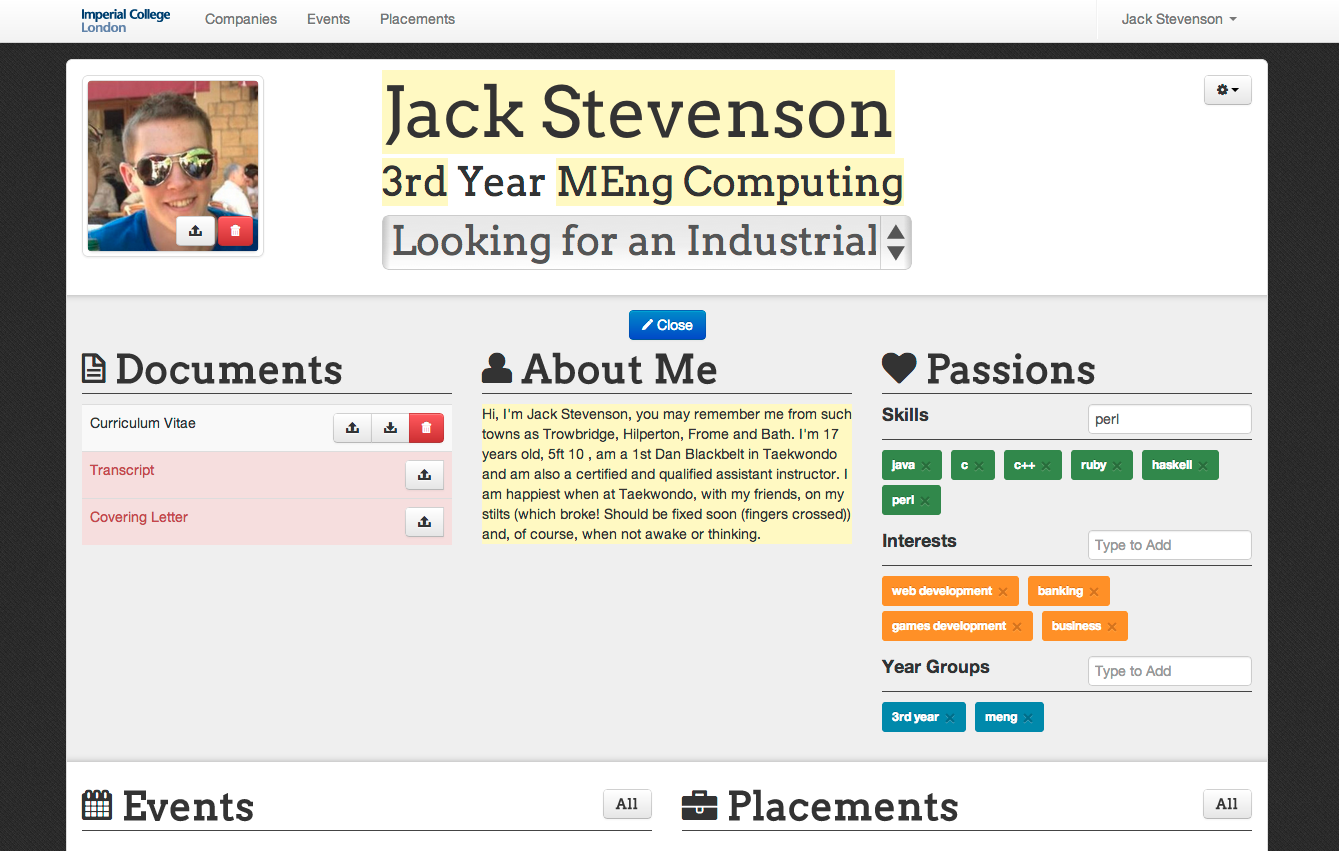
\includegraphics[scale=0.3]{images/user_experiences/student/edit_complete}
    \caption{Completed student profile}
    \end{figure}

    %TODO: Enforce this bug is fixed
    If at any time Jack removes information which is needed in order to make his profile complete it will automatically deactivate and he must complete the information again in order to show up in any company searches.

  \paragraph{Settings:}
    Jack also has an account settings page which can be accessed by clicking on his name which features the navigation bar. Jack can also preview his profile as it appears to companies and log out with this too. 

    Once in his settingds Jack can express if there are any skills or interests he does not wish to receive emails about when looking for a placement, toggle tool tips and company activation, delete his profile or change his password.

    \begin{figure}[H]\centering
    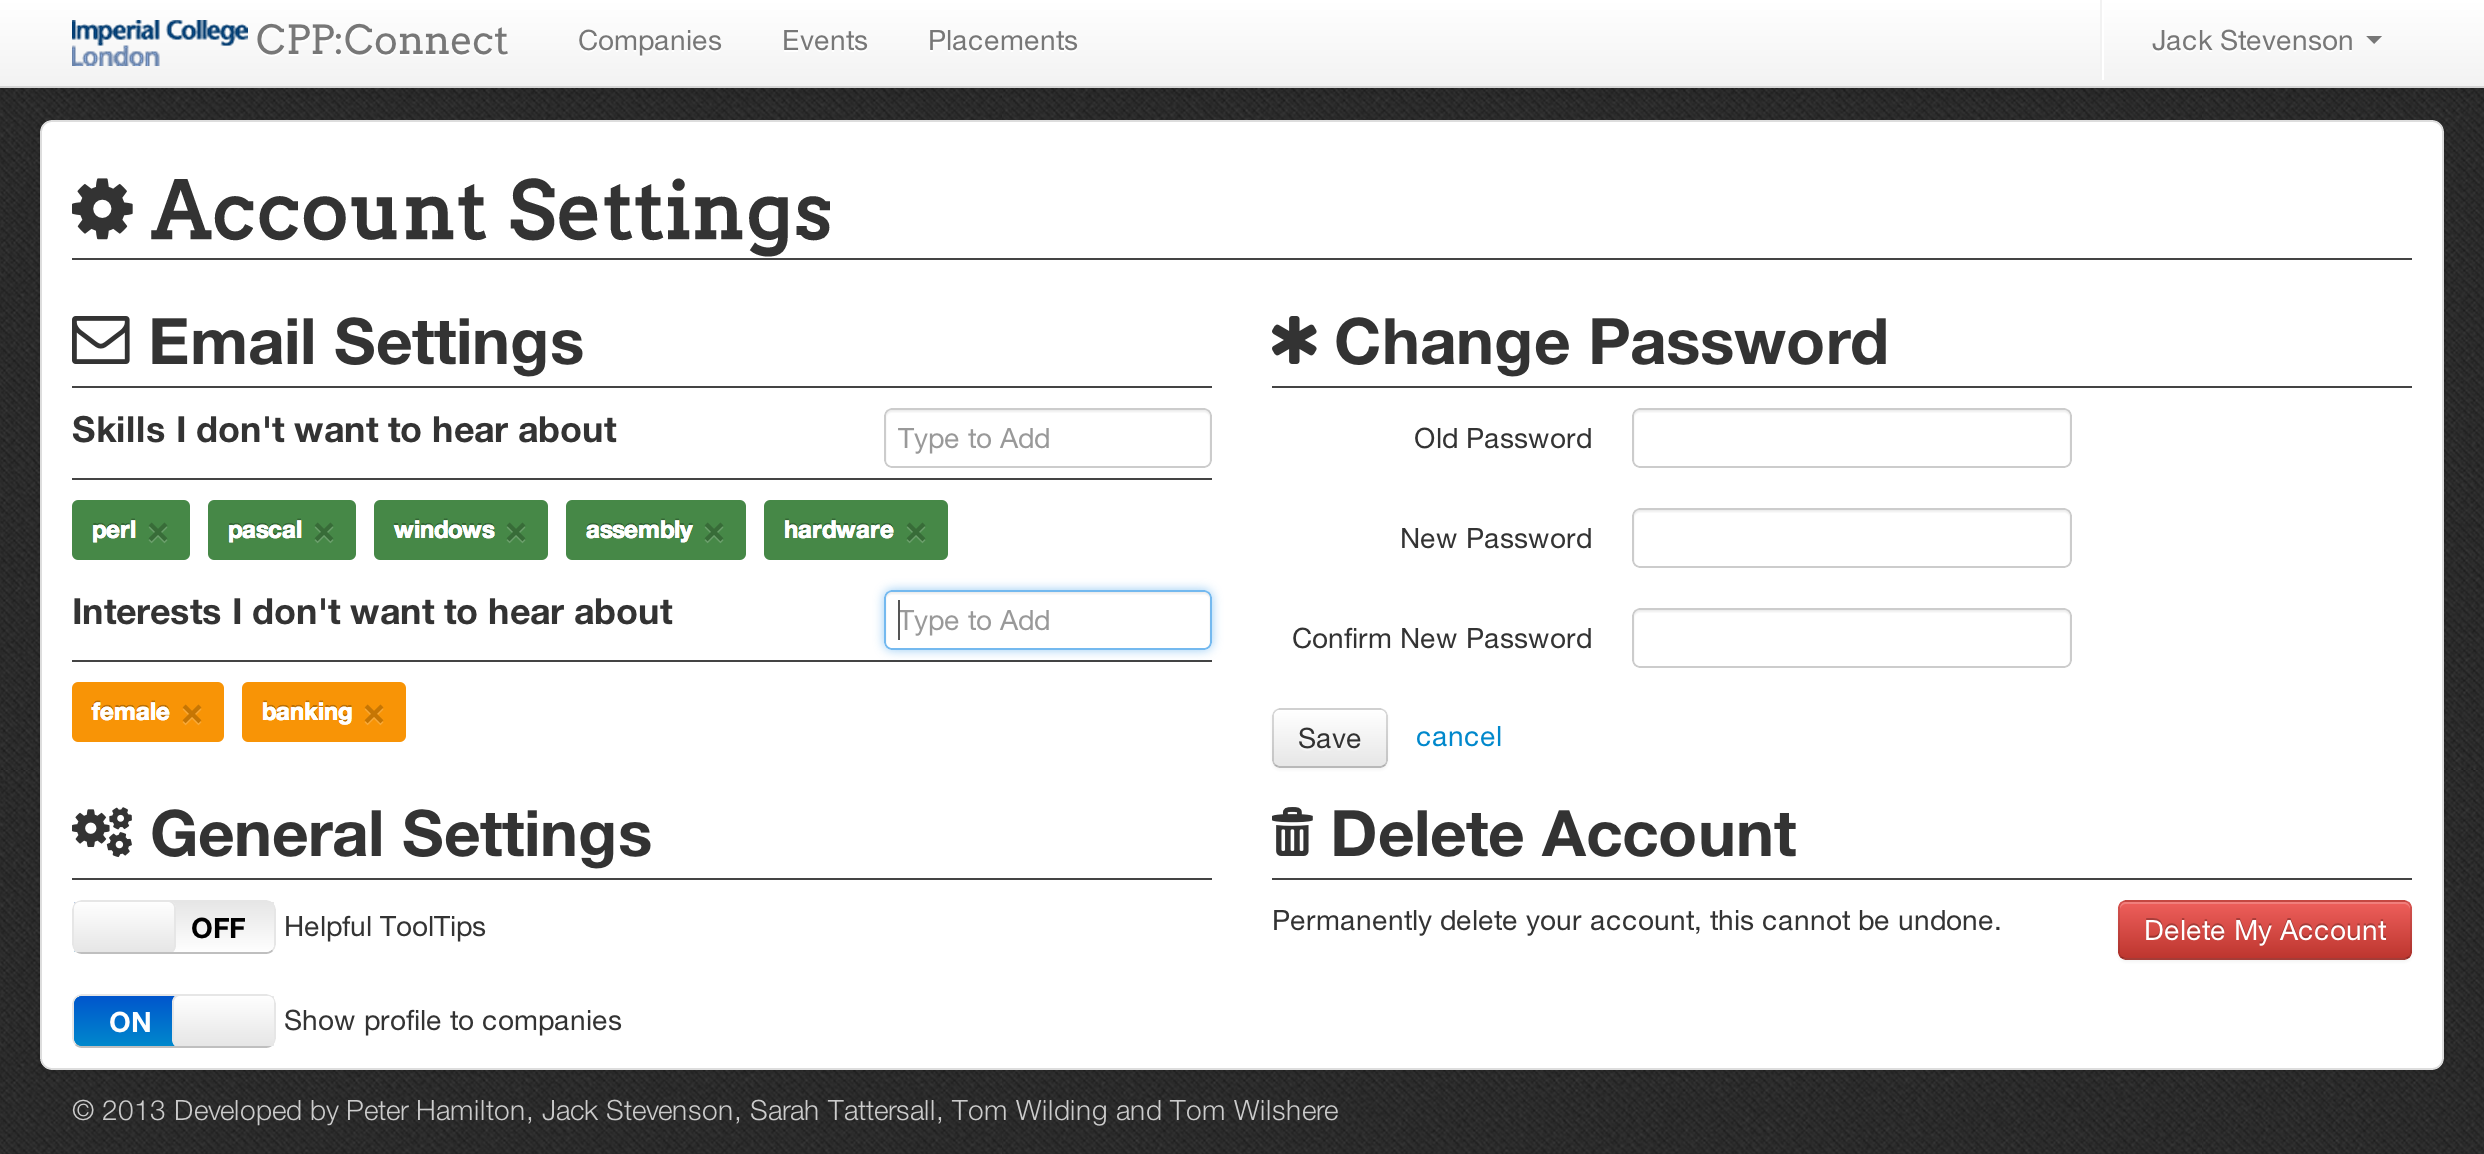
\includegraphics[scale=0.3]{images/user_experiences/student/account_settings}
    \caption{Student settings}
    \end{figure}

    Although we tell students that deleting their account is peremenant, we took the design decision to actually keep old student data in the database unless purged out by the database manager. This is because we may wish to view activity before they deleted themselves or incase a student accidentally deletes themselves and notifies the admin that they've deleted themselves. It would be far nicer if they could be reinstanted, but we don't want to make them aware of this fact because they may loose their cautiousness. We found the rails3\_acts\_as\_paranoid\cite{paranoid_gem} gem took care of this nicely for us and did not require any extra work. It will by default remove `deleted' students from any database queries so that they do not show up on our site.

  \paragraph{Events and Placements:}
    When logged in and looking at his profile, Jack can see new events and placements that have recently been advertised. By attending events students often make better personal contacts with companies than applying online and so Jack may wish to view these events by clicking on any of these or the all button to view the entire list. He can then sign up to attend events and will then receive specific email notifications about them.
    %TODO: PIC HERE
    He can also browse advertised placements and send an email to any companies that advertise any he is really keen about.

    %TODO Pictures about events page and all events and signing up, however not really ready yet.

  \paragraph{Companies:}
    Jack can also browse all companies, finding out a bit more about those he may not have heard of that he might be interested in working for. He does this by clicking on companies on the navigation and can work his way down the list, or choose to filter the list by name and/or description.
    If Jack decides he is not interested in, or does not wish to be contacted by specific companies he can choose to blacklist them. For example if Jack is not interested in a career with Amazon he can search for them on the companies list and then block them with the icon in the corner. He can also faviourte them to make sure he receives information by them, no matter if he has blacklisted a tag (perhaps he might change his mind on Python if it's at the right company?).

    \begin{figure}[H]\centering
    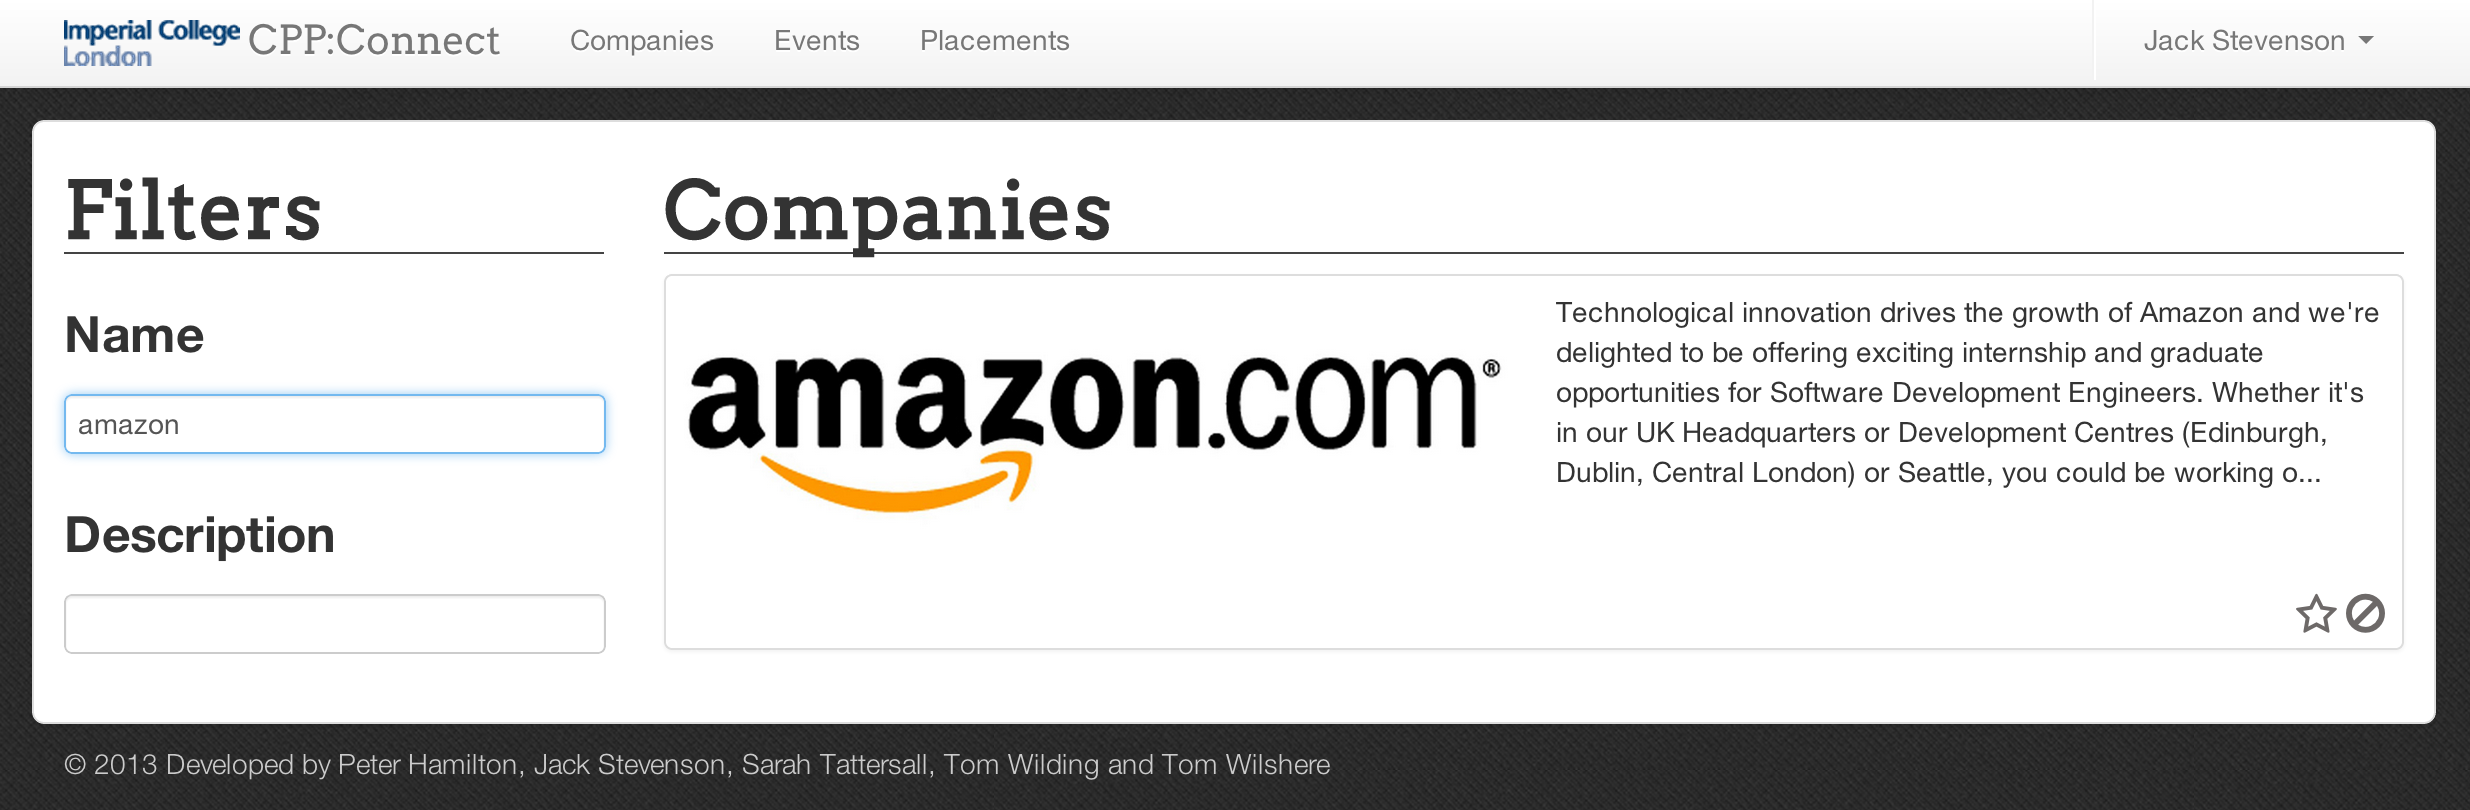
\includegraphics[scale=0.3]{images/user_experiences/student/block_amazon}
    \caption{Students can block or faviourte companies}
    \end{figure}

  \paragraph{Whilst away:}
    Once Jack has finished on the site he can log out and come back any time he wishes to use the it. Whilst away companies can view his profile and he'll receive emails from companies that wish to contact him.

  \paragraph{Later date:}
    If Jack should wish to deactivate his profile in the future, he can easily do so via the deactivation option in his settings, and can re-active it in the exact same manner at a later date. Whilst deactivated Jack can still view and sign up to events as well as view placements and companies. The reason for deactivating is because he does not wish to appear in a company search because either his information is not up to date and will require some time to fix or he has a placement and does not wish to be contacted until he next needs to look for one.

    Should Jack ever forget his password he can click on the `forgot password?' link provided in the navigation bar when he reaches the landing page. This will take him to a form where he registers his email address. Once submitted Jack's password is reset to a secure random eight character password which is automatically generated and is then emailed to him. He is also advised in the email to change his new password straight away, which can be done via the settings page as seen above.